\section{Imagen-Video}
\label{sec:imagen_video}

\begin{figure}
    \centering
    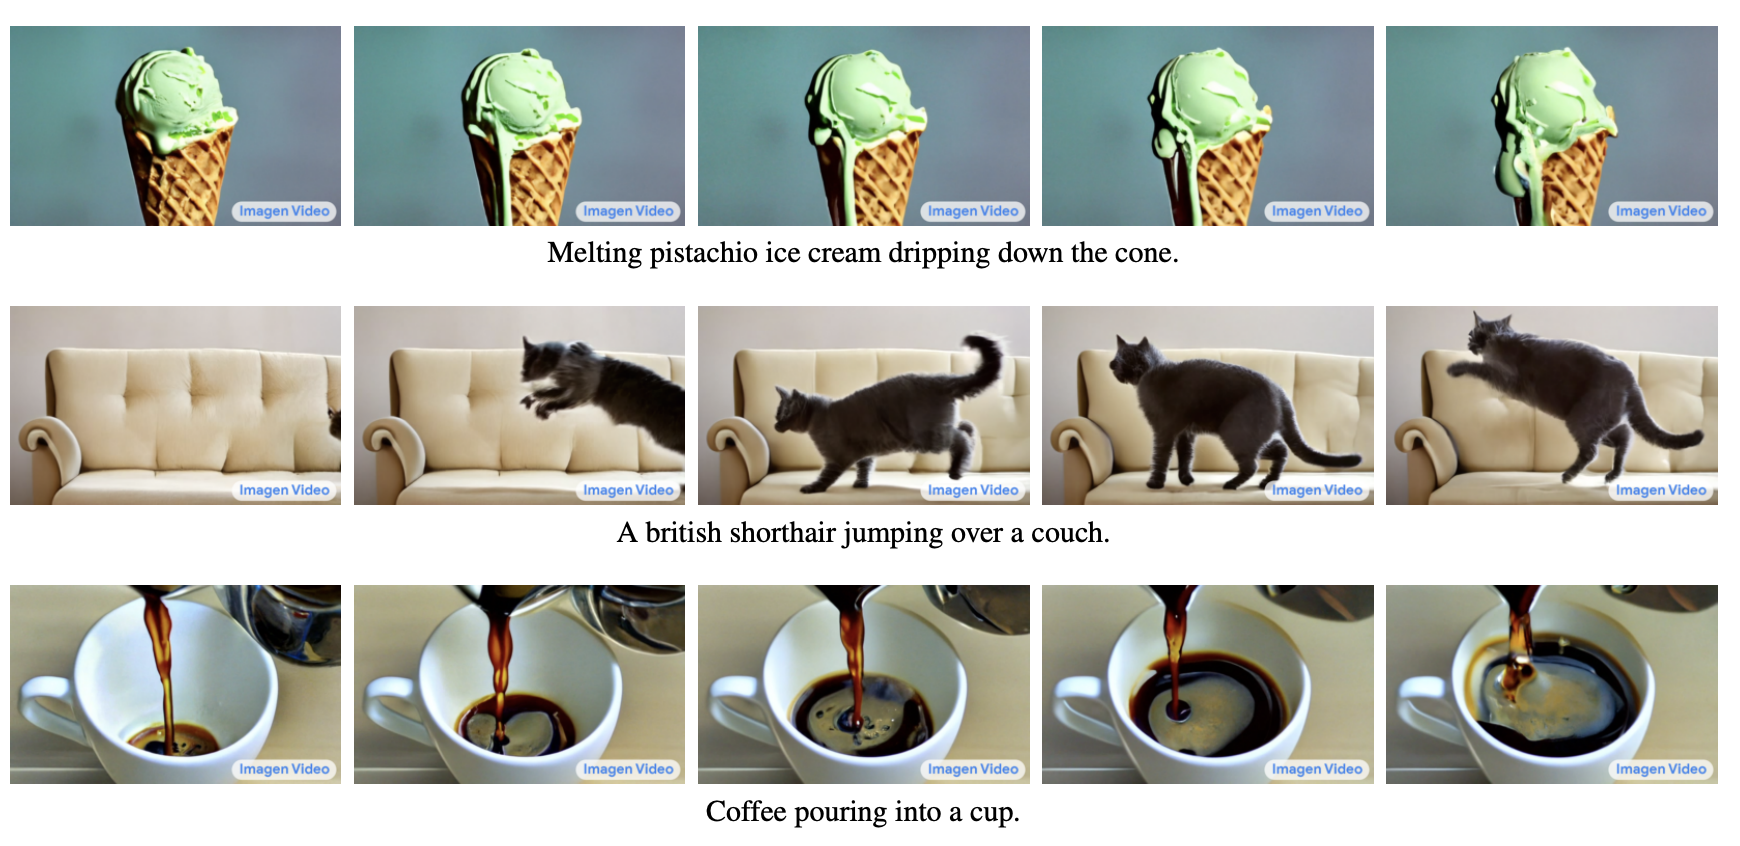
\includegraphics[width=0.7\textwidth]{images/video_synthesis/imagen_video.png}
    \caption{Imagen-Video video samples \cite{imagen_video}.}
\end{figure}

\begin{figure}
    \centering
    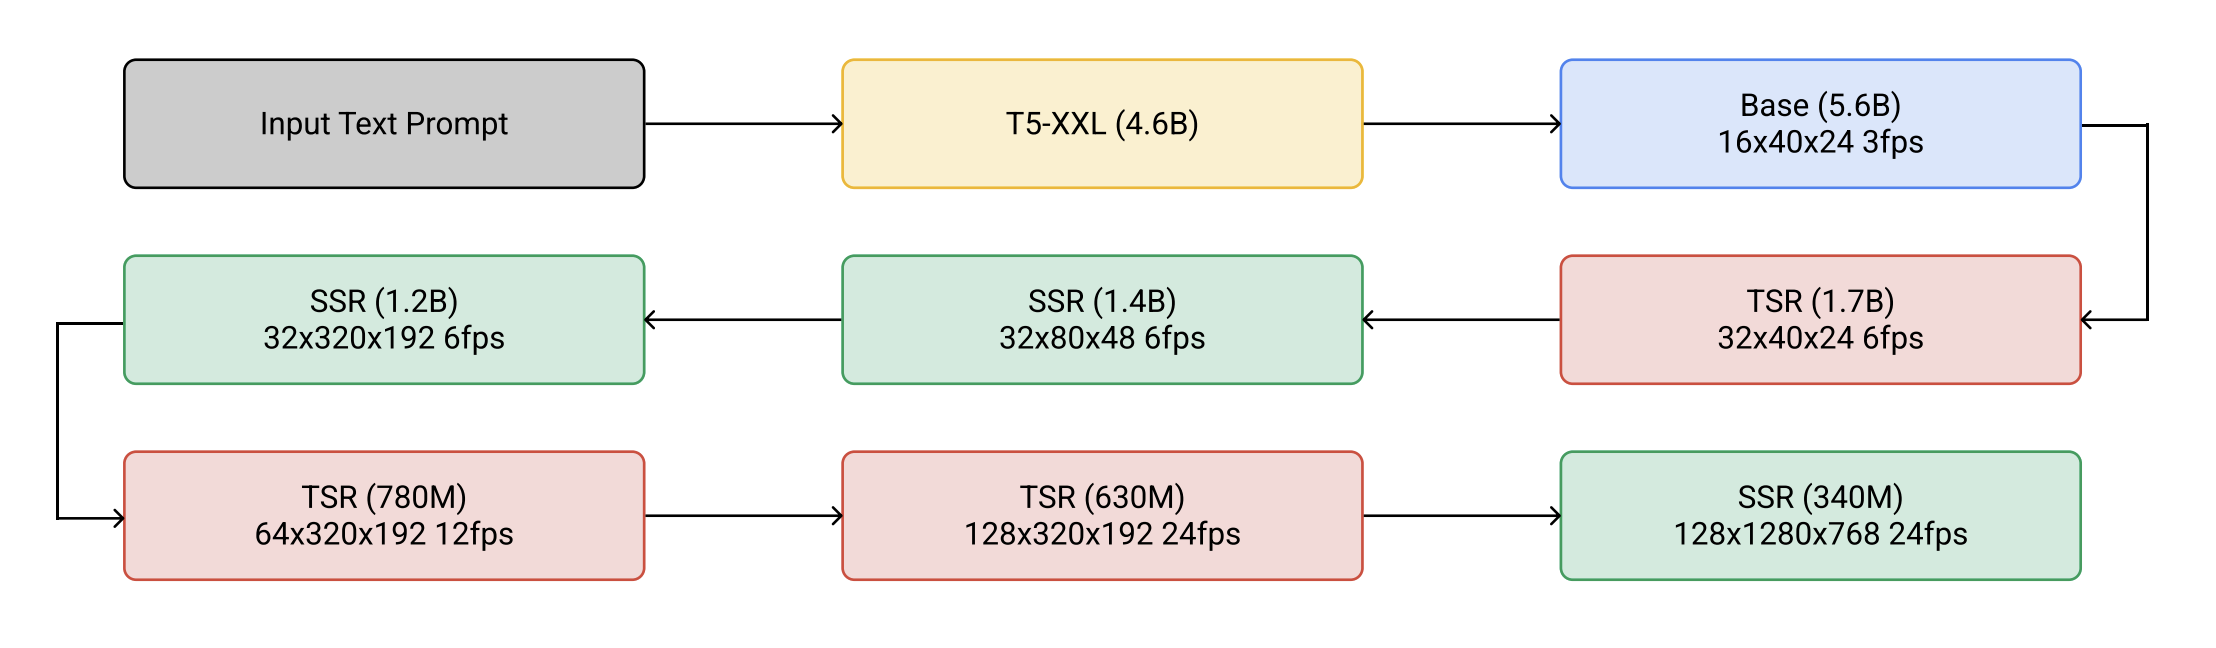
\includegraphics[width=0.7\textwidth]{images/imagen_video/pipeline.png}
    \caption{The cascading pipeline of Imagen-Video. The text embeddings are injected to all models in the pipeline (not shown) \cite{imagen_video}.}
    \label{fig:imagen_video_pipeline}
\end{figure}

Imagen-Video by Google \cite{imagen_video} is a T2V cascading diffusion model, based on Imagen (section \ref{sec:imagen}). Imagen-Video has 7 sub-models in a cascading pipeline (figure \ref{fig:imagen_video_pipeline}). It generates high definition $1280\times 768$ videos @ 24 fps, for 5.3 seconds. A big downside compared to Video-LDM is that Imagen-Video works in the pixel-space, whereas Video-LDM works in latent space. In addition, Imagen-Video is a much larger model and uses more compute resources than Video-LDM, however Google is able to achieve good scaling results through training on massive datasets.

Like Imagen, Imagen-Video uses the same large frozen text-encoder T5-XXL (section \ref{subsec:t5}) in its pipeline. The benefit of cascading pipeline is the ability to independently train each model, allowing the parallel training of all 7 models.

\begin{figure}
    \centering
    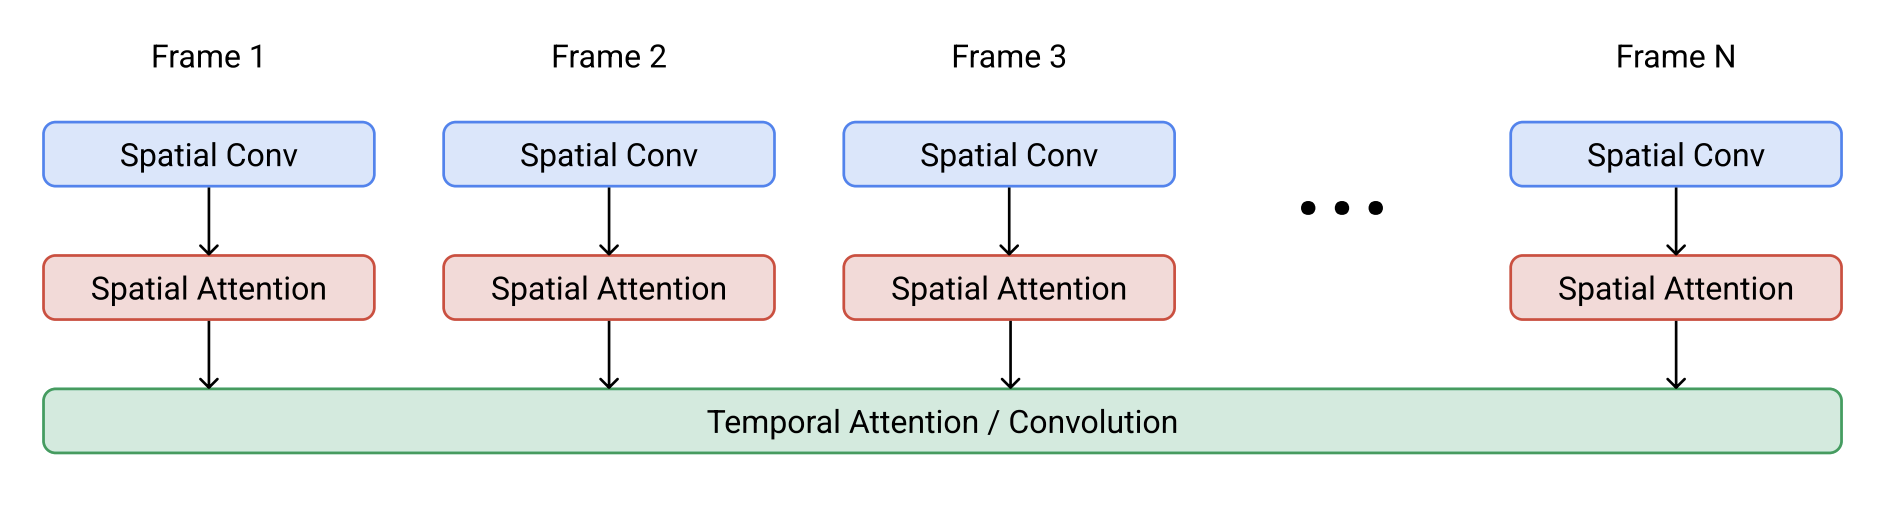
\includegraphics[width=0.7\textwidth]{images/imagen_video/video_u_net.png}
    \caption{Video U-Net block \cite{video_diffusion_models} used by Imagen-Video \cite{imagen_video}.}
    \label{fig:imagen_video_video_unet}
\end{figure}


Imagen Video also builds on the work of \textbf{Video U-Net} \cite{video_diffusion_models}, which generalizes the 2D diffusion model architecture to 3D in space-time by using temporal attention and 3D convolution layers to capture dependencies between video frames. See figure \ref{fig:imagen_video_video_unet}.

Due to safety and ethical concerns in training the Imagen-Video model, the researchers \textbf{decided not to release the model to the public} and keep it closed source.

One of the contribution of the paper is that they successfully transferred multiple methods from the image domain to video, such as \textbf{v-parameterization \cite{v_prediction}, CFG and conditioning augmentation} \cite{cascaded_diffusion_models} (similar to Imagen). They also found out that \textbf{progressive distillation} \cite{v_prediction} \cite{meng2023distillation} is a valuable technique for speeding up video sampling.














\subsection{Architecture \& Method}

Imagen Video has one frozen text encoder (T5-XXL), one base video diffusion model, three SSR (spatial super-resolution) models, and three TSR (temporal super-resolution) models - totaling 7 video diffusion models. Each of the denoising diffusion models $\hat{x_\theta}$ operate on multiple video frames simultaneously. In figure \ref{fig:imagen_video_video_unet} the spatial convolution and spatial attention operate on each frame independently, while temporal attention and convolution operate on a collection of frames.

Whereas typically diffusion models for image generation use a 2D U-Net architecture (spatial attention and convolution), \textbf{Video U-Net} block used by Imagen-Video (figure \ref{fig:imagen_video_video_unet}) generalizes the U-Net to 3D space-time by using temporal attention and convolution to capture dependencies between video frames.

Imagen-Video pipeline is compromised of the following model types:

\begin{itemize}
    \item \textbf{T5-XXL}: T5-XXL is a text-to-text transformer used to encode the text prompts to embeddings which are then used to condition all of the 7 diffusion models.
    \item \textbf{Base}: The base diffusion model generate low FPS low resolution video clip.
    \item \textbf{SSR}: The SSR model is a spatial SR (SSR) model that increases the resolution of the input image. Unlike the base model, it uses temporal convolution instead of temporal attention. Like SR3, we first apply bilinear or bicubic interpolation to increase the resolution, then we remove noise (add details) by first concatenating noise $y_t$ to the upsampled image $x$ and then use the U-Net denoising network to learn to denoise the image.
    \item \textbf{TSR}: The TSR model is a temporal SR (TSR) model that increases the temporal resolution of the input video (increases frame count) by frame interpolation. This model also uses temporal convolution instead of temporal attention.
\end{itemize}

\textbf{Temporal Attention v.s. Temporal Convolution}: Temporal convolution reduces memory and computation costs over temporal attention, which is critical for the SSR and TSR models, because they are applied to high-resolution high-fps videos. This is why temporal attention is used at the beginning of the cascading pipeline.

\textbf{Spatial attention at the beginning of the pipeline}: The base model and the first two SSR models have spatial attention in addition to spatial convolution, because spatial attention at the beginning of the pipeline requires less compute resources than at the end. The last SSR model in the pipeline is a fully convolutional model (without attention).

\textbf{Number of parameters}: Imagen-Video consists of 11.6 billion parameters. Each of the model's parameters count is shown in figure \ref{fig:imagen_video_pipeline}.

\textbf{Classifier-free guidance}: CFG is also used in Imagen-Video. They found that it helps the model generate high fidelity samples with respect to the text prompts. Higher guidance weights lead the model to focus more on the text prompt conditioning.

\textbf{Oscillating guidance}: Similar to Imagen, when the guidance weight is too large, the possible range of values of predicted noise is beyond $[-1, 1]$, which causes train-test mismatch. This leads to significant artifacts in the generated videos. \textbf{Dynamic thresholding}, as described in section \ref{subsec:imagen_diffusion_guidance_weight}, helps to prevent this issue, which dynamically clip the image to the chosen threshold followed by scaling by $s$: \texttt{np.clip(x, -s, s) / s}. However, a constant high guidance weight leads to saturation artifacts, especially at high resolutions. The researchers didn't find dynamic thresholding sufficient, and they experimented with letting the guidance weight \textbf{oscillate between high and low values} (min and max) for a certain number of sampling steps. They apply this \textbf{oscillating dynamic threshold} only to the base and first SR models. The generation starts with a high guidance weight to establish a strong alignment with the prompt, then alternates between high and low weights in subsequent steps.

\textbf{Noise conditioning augmentation}: Similar to Imagen, Imagen-Video applied noise conditioning augmentation for all the spatial and temporal diffusion models. Noise conditioning augmentation is used to \textbf{corrupt low-resolution images}, and then the \textbf{SR model would be conditioned on the noise level}. The corruption noise level ("\textbf{augmentation level}") helps the model to generalize better to various noise levels and improves the diversity and quality of samples. This technique was introduced in a 2021 paper \cite{cascaded_diffusion_models} by Google.







\subsection{Video-image joint training}

Training on both images and videos improves fidelity and enables knowledge transfer from images to videos, addressing the scarcity of text-video pairs datasets. This approach allows the model to learn diverse video styles.

Imagen-Video adopts the joint training method from \cite{video_diffusion_models}, treating individual images as single-frame videos. To exclude temporal components during image training, they mask the temporal computation paths, preventing temporal operations across frames.




















\subsection{v-prediction}

v-prediction (velocity prediction) is a parameterization strategy used in diffusion models to predict the change of pixels in time of the diffusion process. Unlike $\epsilon$-prediction, which the U-Net predicts the noise, v-prediction predicts the change of noise. There is also $x$-prediction in which the U-Net predicts the clean, original data $x_t$ at timestep $t$ instead of the noise added.

v-prediction is defined as:

\[ v \equiv \alpha_t \epsilon - \sigma_t x \]

where $\alpha_t$ is the time-dependent coefficient determined by noise scheduler, $\epsilon$ is the noise, $x$ is the data, and $\sigma_t$ is the standard deviation of the noise at timestep $t$.
















\subsection{Progressive distillation with guidance and stochastic samplers}

In a 2022 paper by Google \cite{v_prediction}, the team introduced \textbf{progressive distillation}, a fast sampling method for diffusion models. Unlike traditional DDPM samplers, requiring thousands of steps, progressive distillation enables sampling in a fixed, reduced number of steps. By iteratively distilling a DDIM sampler (see section \ref{subsec:ddim_sampler}), the required steps are halved with each distillation. This method is used with v-prediction.

\begin{figure}
    \centering
    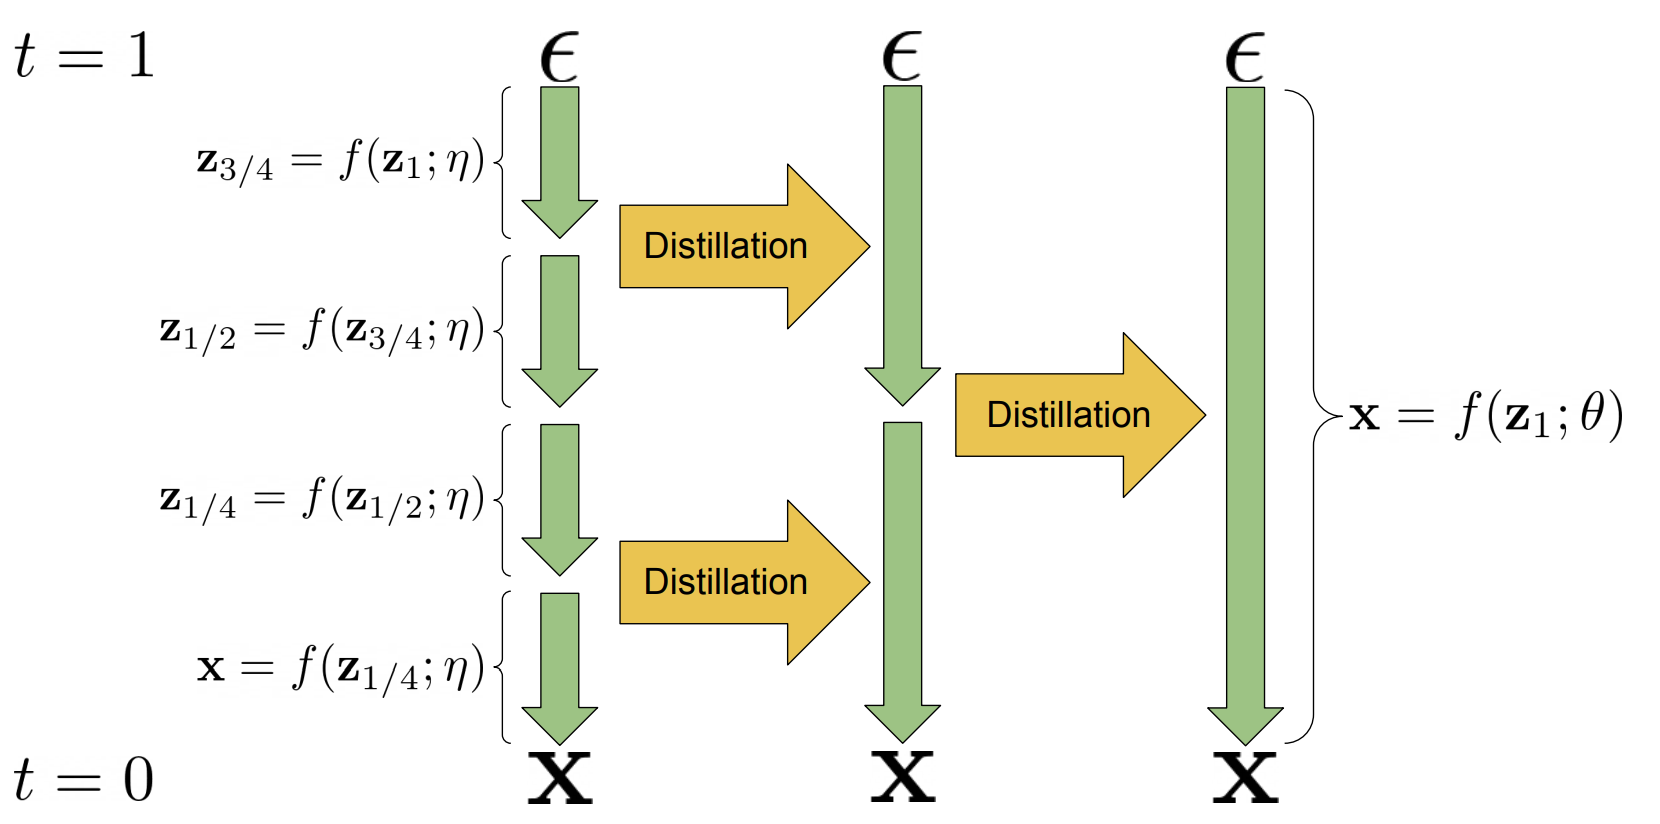
\includegraphics[width=0.6\textwidth]{images/imagen_video/v_prediction.png}
    \caption{Progressive distillation process \cite{v_prediction}.}
    \label{fig:progressive_distillation}
\end{figure}

In figure \ref{fig:progressive_distillation} we see the distillation process: instead of taking 4 sampler steps ($f(z; \eta)$) to transform noise $\epsilon$ to an image $x$, the distilled model now takes a single step.

In progressive distillation we duplicate a model that we desire to distill, which becomes a "student" and "teacher" model (they start with the same weights and biases). The student model learns to produce the output of the teacher model in fewer steps. The teacher model uses two steps of DDIM sampling and the student should learn to output the same teacher's output but in a single sampling step.

% \begin{figure}
%     \centering
%     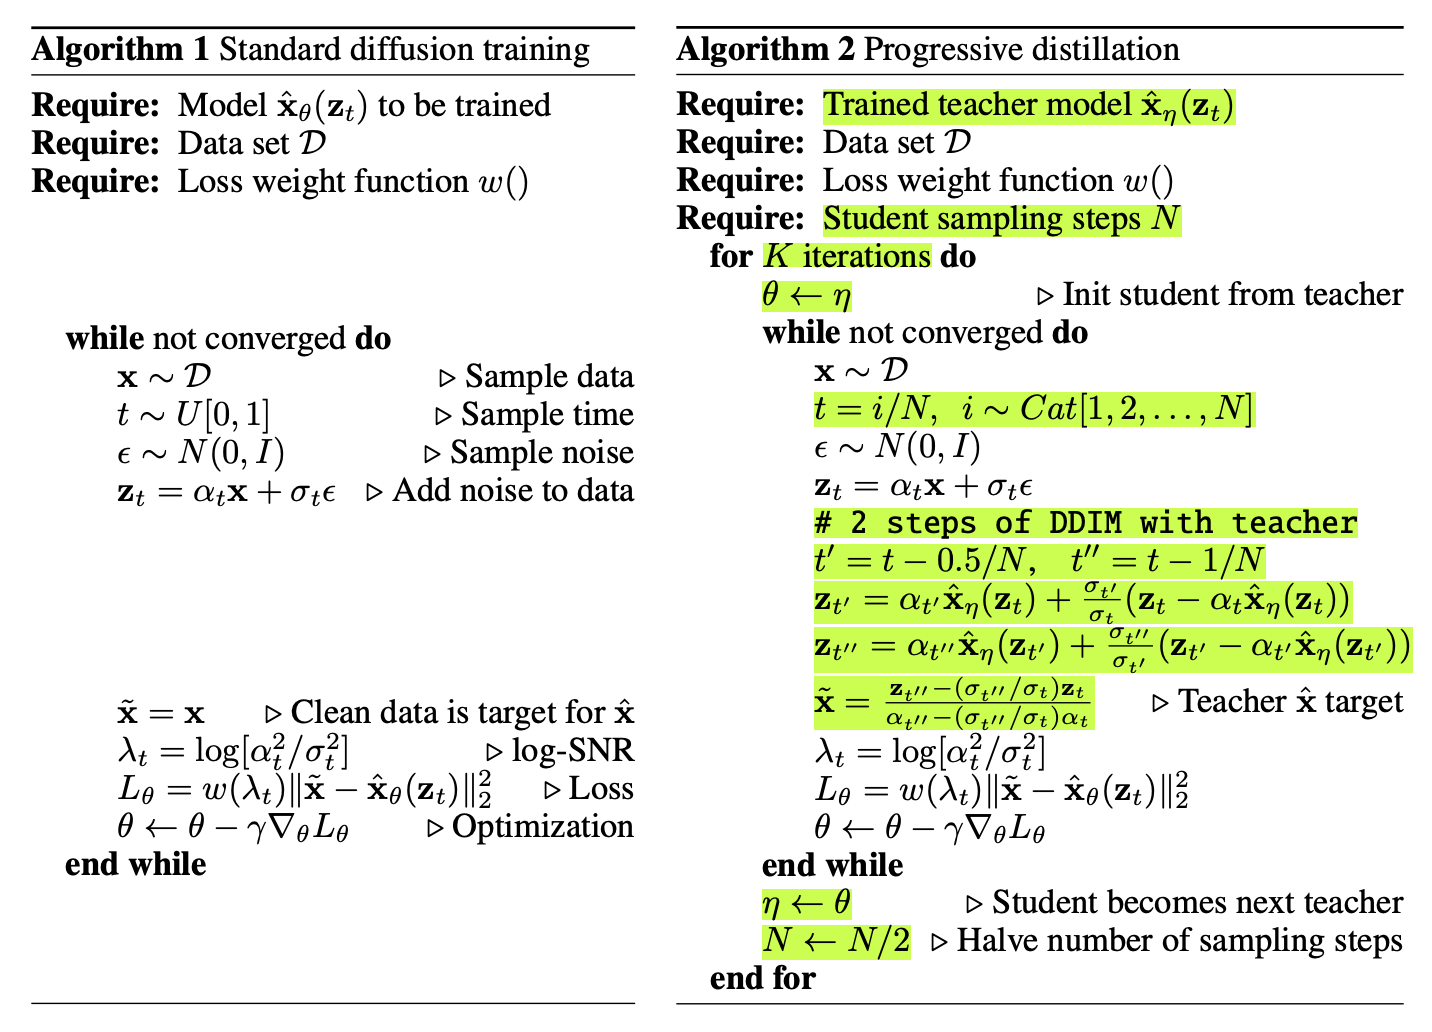
\includegraphics[width=0.7\textwidth]{images/imagen_video/progressive_distillation.png}
%     \caption{Progressive distillation algorithm \cite{v_prediction}. }
%     \label{fig:progressive_distillation_algorithm}
% \end{figure}



\begin{algorithm}[H]
    \centering
    \caption{Standard diffusion training algorithm \cite{v_prediction}}
    \label{alg:ddpm_training_before_distillation}
    \begin{algorithmic}
        \Require Model $\hat{\mathbf{x}}_{\theta}(\mathbf{z}_t)$ to be trained
        \Require Data set $\mathcal{D}$
        \Require Loss weight function $w()$
        
        \While{not converged}
            \State $\mathbf{x} \sim \mathcal{D}$ \Comment{Sample data}
            \State $t \sim U[0,1]$ \Comment{Sample time}
            \State $\epsilon \sim \mathcal{N}(0, I)$ \Comment{Sample noise}
            \State $\mathbf{z}_t = \alpha_t \mathbf{x} + \sigma_t \epsilon$ \Comment{Add noise to data}
            
            \State $\tilde{\mathbf{x}} = \mathbf{x}$ \Comment{Clean data is target for $\hat{\mathbf{x}}$}
            \State $\lambda_t = \log[\alpha_t^2/\sigma_t^2]$ \Comment{log-SNR}
            \State $L_{\theta} = w(\lambda_t) \|\tilde{\mathbf{x}} - \hat{\mathbf{x}}_{\theta}(\mathbf{z}_t)\|_2^2$ \Comment{Loss}
            \State $\theta \gets \theta - \gamma \nabla_{\theta} L_{\theta}$ \Comment{Optimization}
        \EndWhile
    \end{algorithmic}
\end{algorithm}


\begin{algorithm}[H]
    \centering
    \caption{Progressive distillation algorithm \cite{v_prediction}}
    \label{alg:progressive_distillation_algorithm}
    \begin{algorithmic}
        \Require \colorbox{lime} {Trained teacher model $\hat{\mathbf{x}}_{\eta}(\mathbf{z}_t)$}
        \Require Data set $\mathcal{D}$
        \Require Loss weight function $w()$
        \Require \colorbox{lime}{Student sampling steps $N$}
        \For{\colorbox{lime}{$K$ iterations}}
            \State \colorbox{lime}{$\theta \gets \eta$} \Comment{Init student from teacher}
            \While{not converged}
                \State $\mathbf{x} \sim \mathcal{D}$
                \State \colorbox{lime}{$t = i/N, \quad i \sim \text{Cat}[1,2,\dots,N]$}
                \State $\epsilon \sim \mathcal{N}(0, I)$
                \State $\mathbf{z}_t = \alpha_t \mathbf{x} + \sigma_t \epsilon$
                
                \State \colorbox{lime}{{\textbf{\# 2 steps of DDIM with teacher}}}
                \State \colorbox{lime}{{$t' = t - 0.5/N, \quad t'' = t - 1/N$}}
                \State \colorbox{lime}{{$\mathbf{z}_{t'} = \alpha_{t'} \hat{\mathbf{x}}_{\eta}(\mathbf{z}_t) + \frac{\sigma_{t'}}{\sigma_t} (\mathbf{z}_t - \alpha_t \hat{\mathbf{x}}_{\eta}(\mathbf{z}_t))$}}
                \State \colorbox{lime}{{$\mathbf{z}_{t''} = \alpha_{t''} \hat{\mathbf{x}}_{\eta}(\mathbf{z}_{t'}) + \frac{\sigma_{t''}}{\sigma_{t'}} (\mathbf{z}_{t'} - \alpha_{t'} \hat{\mathbf{x}}_{\eta}(\mathbf{z}_{t'}))$}}
                \State \colorbox{lime}{{$\tilde{\mathbf{x}} = \frac{\mathbf{z}_{t''} - (\sigma_{t''}/\sigma_t) \mathbf{z}_t}{\alpha_{t''} - (\sigma_{t''}/\sigma_t) \alpha_t}$}} \Comment{Teacher $\hat{\mathbf{x}}$ target}
                
                \State $\lambda_t = \log[\alpha_t^2/\sigma_t^2]$
                \State $L_{\theta} = w(\lambda_t) \|\tilde{\mathbf{x}} - \hat{\mathbf{x}}_{\theta}(\mathbf{z}_t)\|_2^2$
                \State $\theta \gets \theta - \gamma \nabla_{\theta} L_{\theta}$
            \EndWhile
            \State \colorbox{lime}{$\eta \gets \theta$} \Comment{Student becomes next teacher}
            \State \colorbox{lime}{$N \gets N/2$} \Comment{Halve number of sampling steps}
        \EndFor
    \end{algorithmic}
\end{algorithm}











This process is illustrated in algorithms \ref{alg:progressive_distillation_algorithm} and \ref{alg:ddpm_training_before_distillation}. In algorithm \ref{alg:progressive_distillation_algorithm} the marked lines are the only modifications made to the original training algorithm \ref{alg:ddpm_training_before_distillation} of diffusion models. The teacher model $\hat{x}_{\eta} (z_t)$ is the diffusion model $\hat{x}_{\theta} (z_t)$ where $z_t$ is the noisy data (we take training data $\mathcal{D}$ and add noise to it). After the student model (with parameters $\eta$) learns to predict $\tilde{x}$ (which is two DDIM steps), is distilled to match the output of the teacher model. Then the teacher model becomes the student and the process is repeated.

\begin{figure}
    \centering
    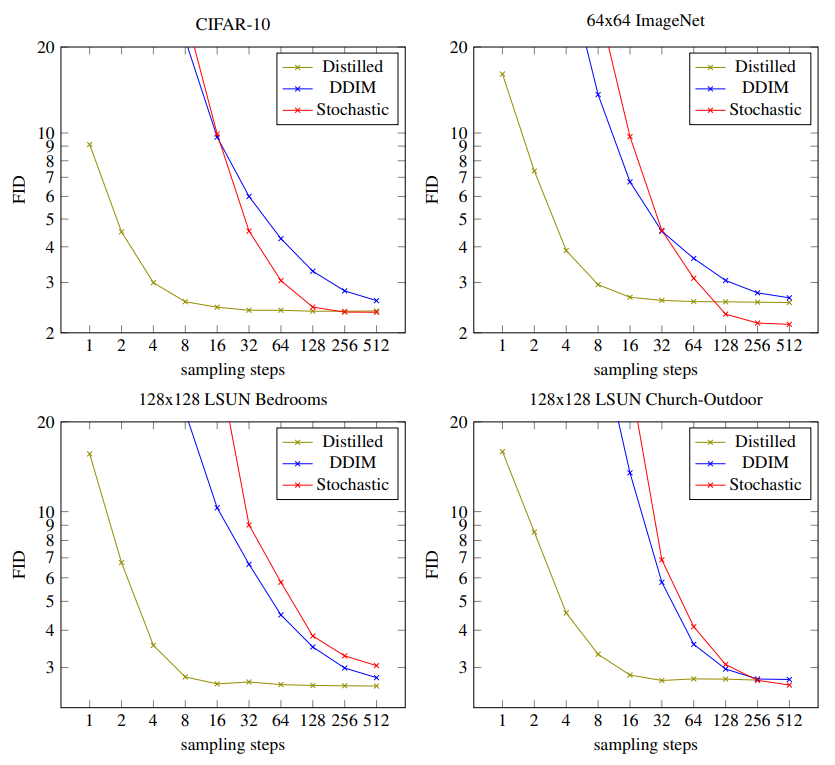
\includegraphics[width=0.6\textwidth]{images/imagen_video/samplers_comparison.png}
    \caption{Comparison of v-prediction sampling to DDIM and stochastic samplers. The distilled model achieves significant lower FID scores with significantly fewer sampling steps (converges faster) \cite{v_prediction}.}
    \label{fig:samplers_comparison}
\end{figure}

We can see in figure \ref{fig:samplers_comparison} that using a distilled model, sampling takes significantly fewer steps to converge to the same quality as the DDIM or stochastic (DDPM) samplers.

\begin{figure}
    \centering
    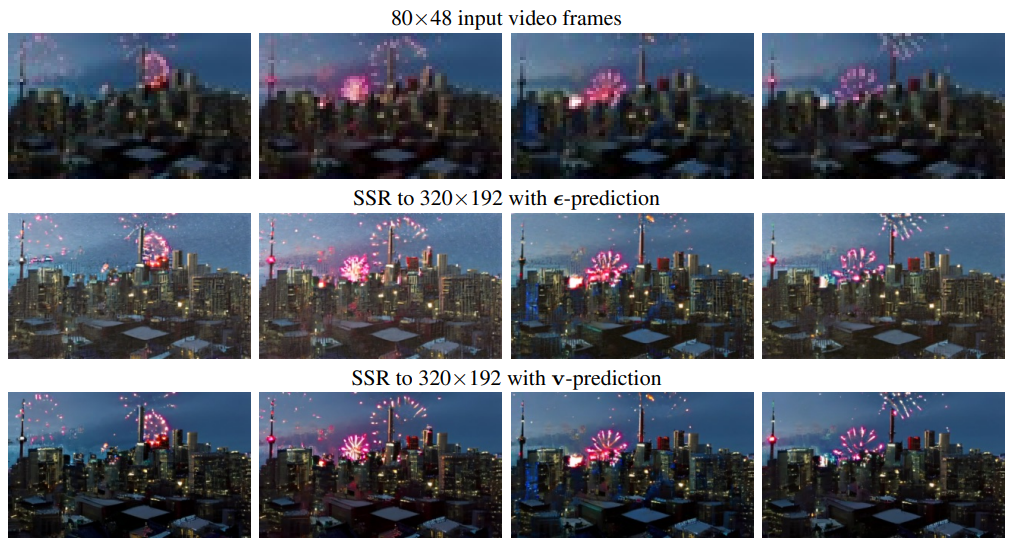
\includegraphics[width=0.7\textwidth]{images/imagen_video/e_prediction_vs_v_prediction.png}
    \caption{$\epsilon$-prediction (middle row) v.s. v-prediction (bottom row). In $\epsilon$-prediction we see color shifts across frames, whereas v-prediction is more consistent \cite{imagen_video}.}
    \label{fig:imagen_video_epsilon_prediction_vs_v_prediction}
\end{figure}

At higher resolutions, v-prediction avoids temporal color shifting artifacts compared to $\epsilon$-prediction. We can see that in figure \ref{fig:imagen_video_epsilon_prediction_vs_v_prediction}. The researchers say the reason is that in distillation we have to work at higher noise levels to the point where the signal-to-noise ratio (SNR) drops to zero, at which point predicting the noise becomes a lot harder.













\subsubsection*{Distillation with classifier-free guidance}

The paper \cite{meng2023distillation} by Google Research and Stability AI extends \cite{v_prediction} by applying distillation to models trained with CFG, marking its first use in video domain. In this work, the teacher model (trained with CFG, before distillation) takes two DDIM steps, and the student model, denoted in the paper as a $w$-conditioned model, learns to match the teacher's output while being conditioned on the guidance scale. This conditioning incorporates the guidance weight into the model backbone, similar to timestep conditioning in \cite{kingma2021variational}. The student model is optimized with the following objective \cite{meng2023distillation}:

\begin{equation*}
\mathbb{E}_{w \sim p_w, t \sim U[0, 1], x \sim p_{\text{data}}(x)} 
\left[ 
    \omega(\lambda_t) \left\| 
        \underbrace{\hat{x}_{\eta_1}(z_t, w)}_{\text{student's pred}} - 
        \underbrace{\hat{x}_{\theta}^w(z_t) }_{\text{teacher's pred}}
    \right\|_2^2 
\right]
\end{equation*}

where:

\begin{itemize}
    \item $w$ is the guidance weight and is picked from $p_w$: $w \sim p_w$ (which can be fixed or oscillate, but in Imagen-Video they chose to oscillate)
    \item $p_w(w) = U[w_{\text{min}}, w_{\text{max}}]$ is the oscillating guidance weight function
    \item $t$ is the diffusion timestep
    \item $x$ is the data (images): $x \sim p_{\text{data}}(x)$
    \item $z_t$ is the noised version of $x$ (noisy image at timestep $t$)
    \item $\lambda_t$ is the guidance scale (not really important)
    \item $\omega(\lambda_t)$ is the weighting function (also not really important)
    \item $\hat{x}_{\eta_1}$ is the student model (which is conditioned on the guidance weight $w$ as input: $\hat{x}_{\eta_1}(z_t, \textcolor{red}{w})$). Also notice the notation: $\hat{x}_{\eta_\mathbf{\textcolor{red}{1}}}$, which means that this is the first distillation iteration.
    \item $\hat{x}_{\theta}^w$ is the teacher model. Notice in the notation, it is using the guidance weight in CFG (it is not given as input): $\hat{x}_{\theta}^\mathbf{\textcolor{red}{w}}(z_t)$
\end{itemize}

Also notice that the teacher model's parameters ($\eta$) are different to the student model's parameters ($\theta$), since they change at each distillation step (the student is a copy of the teacher but to differentiate between the parameters after the distillation process they chose to differentiate the parameters notations).

In the \cite{meng2023distillation} paper we optimize the student's objective:

\[  
    \hat{x}_{\theta}^w(z_t) = 
    \underbrace{(1+w) \hat{x}_{c,\theta} (z_t)}_{\text{conditional score}} - 
    \underbrace{w \hat{x}_\theta (z_t)}_{\text{unconditional score}}
\]

where $c$ is the teacher model's conditioning (for example, text prompt)\footnote{Thanks to \href{https://www.youtube.com/watch?v=ZXuK6IRJlnk}{this youtube tutorial} for explaining both papers}.

To summarize, Using the work of \cite{meng2023distillation}, Imagen-Video researchers successfully distilled 7 video diffusion models with CFG to just 8 sampling steps without any noticeable loss in perceptual quality in the pipeline.

















\subsection{Experiments}

In their experiments, they sampled video clips at $192\times 320$ resolution @ 24 fps for 128 frames (5.3 seconds). They repeat the evaluations over four runs and report the mean and standard error.

\textbf{Datasets}: The researchers used 14 billion video-text pairs and 60 million image-text pairs from internal and public datasets, such as LAION-400M \cite{laion_400m}.

\textbf{Pre-processing}: They resized images using antialiased bilinear resizing and temporally resize videos by skipping frames.

\textbf{Evaluation}: They used FID on individual video frames, FVD for video, and frame-wise CLIP scores for video-text alignment (they take the average across all frames).

\begin{figure}
    \centering
    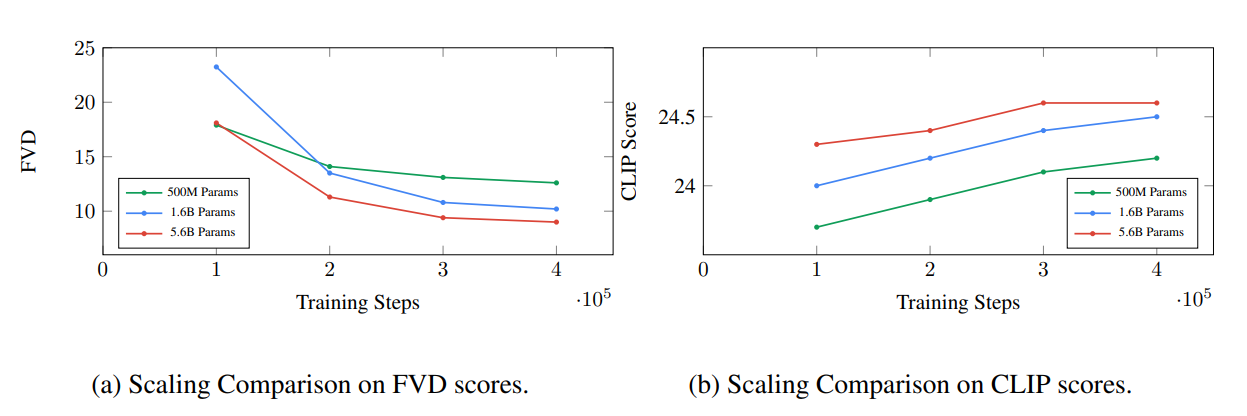
\includegraphics[width=0.8\textwidth]{images/imagen_video/scaling.png}
    \caption{Imagen-Video scaling results on video U-Net. The more parameters the model has, the better the FVD and CLIP scores \cite{imagen_video}.}
    \label{fig:imagen_video_scaling}
\end{figure}

\textbf{Scaling}: In figure \ref{fig:imagen_video_scaling} we can see interesting result which contradicts the findings of Imagen \cite{imagen} paper. They found that increasing the U-Net size doesn't scale the sample quality as much as increasing the text encoder size. They conclude that video modeling task for which the performance is not yet saturated at current model sizes\footnote{This finding could hint that transformers, which benefit from scaling on large datasets, could provide the necessary scaling capabilities that video modeling task demands.}.

\begin{figure}
    \centering
    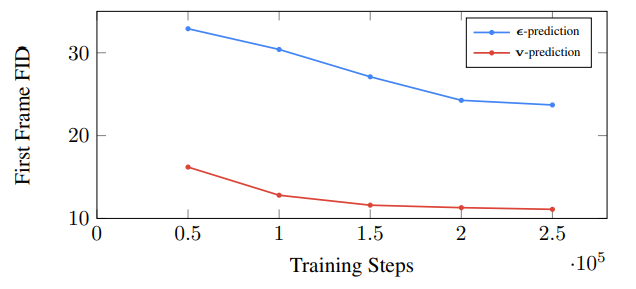
\includegraphics[width=0.5\textwidth]{images/imagen_video/e_prediction_vs_v_prediction_2.png}
    \caption{$\epsilon$-prediction v.s. v-prediction parameterization. v-prediction converges faster \cite{imagen_video}.}
\end{figure}

\begin{figure}
    \centering
    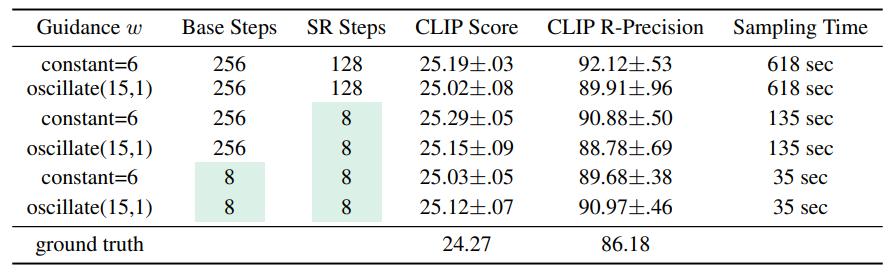
\includegraphics[width=0.6\textwidth]{images/imagen_video/experiments_table.png}
    \caption{Testing of fixed and oscillating guidance weight, distillation of base and SR models and evaluating each pipeline on CLIP score and sampling time. Distilling the pipeline results in significantly faster sampling time, while oscillating guidance weight improves the CLIP score a little \cite{imagen_video}.}
    \label{fig:imagen_video_experiments_table}
\end{figure}

\textbf{Quality vs. Sampling time in a distilled model}: In figure \ref{fig:imagen_video_experiments_table} we can see that distillation provides a good trade-off between sampling time and quality. Distilled model is 18x times faster in sampling, without significant degradation in perceptual quality. IIn addition, the distilled model is also 36x more efficient in terms of compute cost in FLOPs metric. 

